\documentclass[tikz]{standalone}

\usetikzlibrary{automata,positioning,calc}

\begin{document}
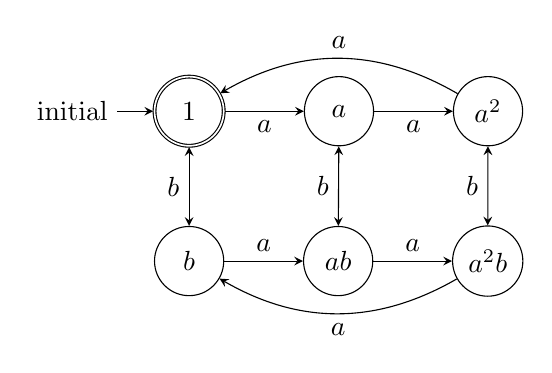
\begin{tikzpicture}[>=stealth,node distance=1,initial text={initial}]

\node [state,initial,accepting] (one) {$1$};

\node[state] (a) [right=of one]{$a$};
\node[state] (aa) [right=of a]{$a^2$};

\node[state] (b) [below=of one]{$b$};
\node[state] (ba) [right=of b]{$ab$};
\node[state] (baa) [right=of ba]{$a^2b$};

\path[->]
	(one) edge node [below] {$a$} (a)
	(a) edge node [below] {$a$} (aa)
	(b) edge node [above] {$a$} (ba)
	(ba) edge node [above] {$a$} (baa)
	(aa) edge[bend right] node [above] {$a$} (one)
	(baa) edge[bend left] node[below] {$a$} (b)
;

\path[<->]
	(one) edge node [left] {$b$} (b)
	(a) edge node [left] {$b$} (ba)
	(aa) edge node [left] {$b$} (baa)
;

\end{tikzpicture}
\end{document}
